\documentclass{standalone}
\usepackage{tikz}
\usetikzlibrary{patterns, positioning}


\begin{document}
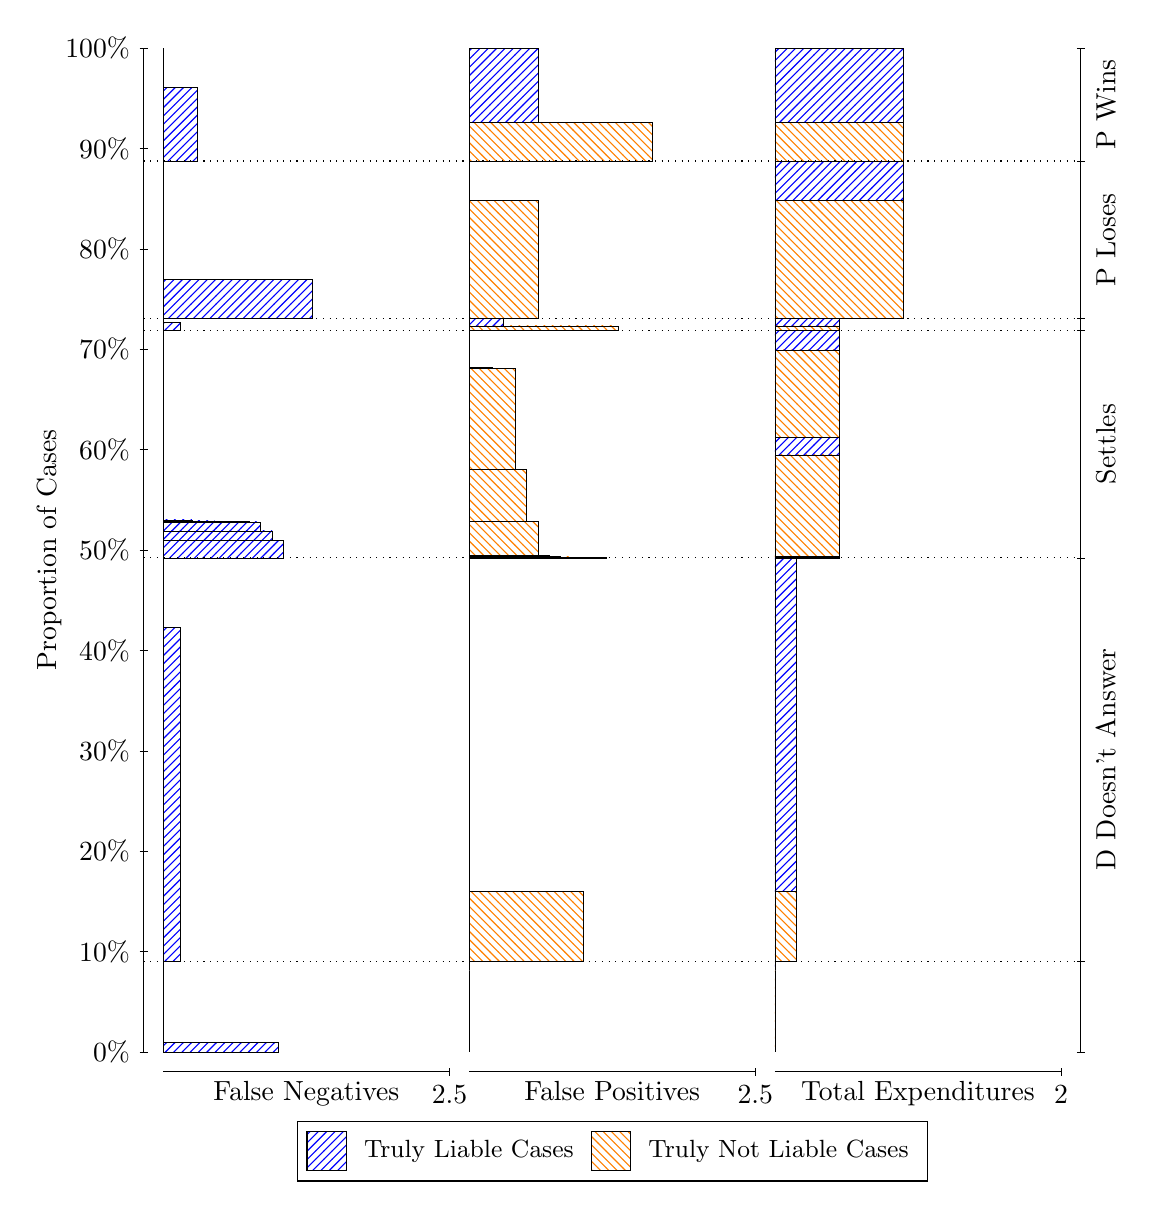
\begin{tikzpicture}
\draw[black, very thin] (1.5,1.75) -- (1.5,14.5);
\node[rotate=90, text=black, anchor=center] at (0.3, 8.125) {Proportion of Cases};
\draw[black, very thin] (1.45,1.75) -- (1.55,1.75);
\node[text=black, anchor=east] at (1.45, 1.75) {0\%};
\draw[black, very thin] (1.45,3.025) -- (1.55,3.025);
\node[text=black, anchor=east] at (1.45, 3.025) {10\%};
\draw[black, very thin] (1.45,4.3) -- (1.55,4.3);
\node[text=black, anchor=east] at (1.45, 4.3) {20\%};
\draw[black, very thin] (1.45,5.575) -- (1.55,5.575);
\node[text=black, anchor=east] at (1.45, 5.575) {30\%};
\draw[black, very thin] (1.45,6.85) -- (1.55,6.85);
\node[text=black, anchor=east] at (1.45, 6.85) {40\%};
\draw[black, very thin] (1.45,8.125) -- (1.55,8.125);
\node[text=black, anchor=east] at (1.45, 8.125) {50\%};
\draw[black, very thin] (1.45,9.4) -- (1.55,9.4);
\node[text=black, anchor=east] at (1.45, 9.4) {60\%};
\draw[black, very thin] (1.45,10.675) -- (1.55,10.675);
\node[text=black, anchor=east] at (1.45, 10.675) {70\%};
\draw[black, very thin] (1.45,11.95) -- (1.55,11.95);
\node[text=black, anchor=east] at (1.45, 11.95) {80\%};
\draw[black, very thin] (1.45,13.225) -- (1.55,13.225);
\node[text=black, anchor=east] at (1.45, 13.225) {90\%};
\draw[black, very thin] (1.45,14.5) -- (1.55,14.5);
\node[text=black, anchor=east] at (1.45, 14.5) {100\%};

\draw[black, very thin] (13.4,1.75) -- (13.4,14.5);
\draw[black, very thin] (13.35,1.75) -- (13.45,1.75);
\node[anchor=west] at (13.35, 1.75) {};
\draw[black, very thin] (13.35,2.9038) -- (13.45,2.9038);
\node[anchor=west] at (13.35, 2.9038) {};
\draw[black, very thin] (13.35,8.0244) -- (13.45,8.0244);
\node[anchor=west] at (13.35, 8.0244) {};
\draw[black, very thin] (13.35,10.918) -- (13.45,10.918);
\node[anchor=west] at (13.35, 10.918) {};
\draw[black, very thin] (13.35,11.064) -- (13.45,11.064);
\node[anchor=west] at (13.35, 11.064) {};
\draw[black, very thin] (13.35,13.065) -- (13.45,13.065);
\node[anchor=west] at (13.35, 13.065) {};
\draw[black, very thin] (13.35,14.5) -- (13.45,14.5);
\node[anchor=west] at (13.35, 14.5) {};

\draw[black, very thin, pattern color=blue, pattern=north east lines] (1.75,1.75) rectangle (3.2033,1.8714);
\draw[black, very thin, pattern color=orange, pattern=north west lines] (1.75,1.8714) rectangle (1.75,2.9038);
\draw[black, very thin, pattern color=blue, pattern=north east lines] (1.75,2.9038) rectangle (1.968,7.1405);
\draw[black, very thin, pattern color=orange, pattern=north west lines] (1.75,7.1405) rectangle (1.75,8.0244);
\draw[black, very thin, pattern color=blue, pattern=north east lines] (1.75,8.0244) rectangle (3.276,8.2486);
\draw[black, very thin, pattern color=blue, pattern=north east lines] (1.75,8.2486) rectangle (3.1307,8.3676);
\draw[black, very thin, pattern color=blue, pattern=north east lines] (1.75,8.3676) rectangle (2.9853,8.4816);
\draw[black, very thin, pattern color=blue, pattern=north east lines] (1.75,8.4816) rectangle (2.84,8.4857);
\draw[black, very thin, pattern color=blue, pattern=north east lines] (1.75,8.4857) rectangle (2.6947,8.4901);
\draw[black, very thin, pattern color=blue, pattern=north east lines] (1.75,8.4901) rectangle (2.5493,8.4926);
\draw[black, very thin, pattern color=blue, pattern=north east lines] (1.75,8.4926) rectangle (2.404,8.4942);
\draw[black, very thin, pattern color=blue, pattern=north east lines] (1.75,8.4942) rectangle (2.2587,8.496);
\draw[black, very thin, pattern color=blue, pattern=north east lines] (1.75,8.496) rectangle (2.1133,8.5085);
\draw[black, very thin, pattern color=orange, pattern=north west lines] (1.75,8.5085) rectangle (1.75,10.918);
\draw[black, very thin, pattern color=blue, pattern=north east lines] (1.75,10.918) rectangle (1.968,11.013);
\draw[black, very thin, pattern color=orange, pattern=north west lines] (1.75,11.013) rectangle (1.75,11.064);
\draw[black, very thin, pattern color=blue, pattern=north east lines] (1.75,11.064) rectangle (3.6393,11.563);
\draw[black, very thin, pattern color=orange, pattern=north west lines] (1.75,11.563) rectangle (1.75,13.065);
\draw[black, very thin, pattern color=blue, pattern=north east lines] (1.75,13.065) rectangle (2.186,14.004);
\draw[black, very thin, pattern color=orange, pattern=north west lines] (1.75,14.004) rectangle (1.75,14.5);
\draw[black, very thin, pattern color=orange, pattern=north west lines] (5.6333,1.75) rectangle (5.6333,2.7824);
\draw[black, very thin, pattern color=blue, pattern=north east lines] (5.6333,2.7824) rectangle (5.6333,2.9038);
\draw[black, very thin, pattern color=orange, pattern=north west lines] (5.6333,2.9038) rectangle (7.0867,3.7877);
\draw[black, very thin, pattern color=blue, pattern=north east lines] (5.6333,3.7877) rectangle (5.6333,8.0244);
\draw[black, very thin, pattern color=orange, pattern=north west lines] (5.6333,8.0244) rectangle (7.3773,8.0301);
\draw[black, very thin, pattern color=orange, pattern=north west lines] (5.6333,8.0301) rectangle (7.232,8.0319);
\draw[black, very thin, pattern color=orange, pattern=north west lines] (5.6333,8.0319) rectangle (7.0867,8.0336);
\draw[black, very thin, pattern color=orange, pattern=north west lines] (5.6333,8.0336) rectangle (6.9413,8.0377);
\draw[black, very thin, pattern color=orange, pattern=north west lines] (5.6333,8.0377) rectangle (6.796,8.0472);
\draw[black, very thin, pattern color=orange, pattern=north west lines] (5.6333,8.0472) rectangle (6.6507,8.0559);
\draw[black, very thin, pattern color=orange, pattern=north west lines] (5.6333,8.0559) rectangle (6.5053,8.4845);
\draw[black, very thin, pattern color=orange, pattern=north west lines] (5.6333,8.4845) rectangle (6.36,9.1463);
\draw[black, very thin, pattern color=orange, pattern=north west lines] (5.6333,9.1463) rectangle (6.2147,10.434);
\draw[black, very thin, pattern color=blue, pattern=north east lines] (5.6333,10.434) rectangle (5.924,10.447);
\draw[black, very thin, pattern color=blue, pattern=north east lines] (5.6333,10.447) rectangle (5.7787,10.449);
\draw[black, very thin, pattern color=blue, pattern=north east lines] (5.6333,10.449) rectangle (5.6333,10.918);
\draw[black, very thin, pattern color=orange, pattern=north west lines] (5.6333,10.918) rectangle (7.5227,10.97);
\draw[black, very thin, pattern color=blue, pattern=north east lines] (5.6333,10.97) rectangle (6.0693,11.064);
\draw[black, very thin, pattern color=orange, pattern=north west lines] (5.6333,11.064) rectangle (6.5053,12.566);
\draw[black, very thin, pattern color=blue, pattern=north east lines] (5.6333,12.566) rectangle (5.6333,13.065);
\draw[black, very thin, pattern color=orange, pattern=north west lines] (5.6333,13.065) rectangle (7.9587,13.56);
\draw[black, very thin, pattern color=blue, pattern=north east lines] (5.6333,13.56) rectangle (6.5053,14.5);
\draw[black, very thin, pattern color=orange, pattern=north west lines] (9.5167,1.75) rectangle (9.5167,2.7824);
\draw[black, very thin, pattern color=blue, pattern=north east lines] (9.5167,2.7824) rectangle (9.5167,2.9038);
\draw[black, very thin, pattern color=orange, pattern=north west lines] (9.5167,2.9038) rectangle (9.7892,3.7877);
\draw[black, very thin, pattern color=blue, pattern=north east lines] (9.5167,3.7877) rectangle (9.7892,8.0244);
\draw[black, very thin, pattern color=orange, pattern=north west lines] (9.5167,8.0244) rectangle (10.334,8.0373);
\draw[black, very thin, pattern color=blue, pattern=north east lines] (9.5167,8.0373) rectangle (10.334,8.0452);
\draw[black, very thin, pattern color=orange, pattern=north west lines] (9.5167,8.0452) rectangle (10.334,9.3332);
\draw[black, very thin, pattern color=blue, pattern=north east lines] (9.5167,9.3332) rectangle (10.334,9.5573);
\draw[black, very thin, pattern color=orange, pattern=north west lines] (9.5167,9.5573) rectangle (10.334,10.666);
\draw[black, very thin, pattern color=blue, pattern=north east lines] (9.5167,10.666) rectangle (10.334,10.918);
\draw[black, very thin, pattern color=orange, pattern=north west lines] (9.5167,10.918) rectangle (10.334,10.97);
\draw[black, very thin, pattern color=blue, pattern=north east lines] (9.5167,10.97) rectangle (10.334,11.064);
\draw[black, very thin, pattern color=orange, pattern=north west lines] (9.5167,11.064) rectangle (11.152,12.566);
\draw[black, very thin, pattern color=blue, pattern=north east lines] (9.5167,12.566) rectangle (11.152,13.065);
\draw[black, very thin, pattern color=orange, pattern=north west lines] (9.5167,13.065) rectangle (11.152,13.56);
\draw[black, very thin, pattern color=blue, pattern=north east lines] (9.5167,13.56) rectangle (11.152,14.5);
\draw[black, dotted] (1.5,2.9038) -- (13.4,2.9038);
\draw[black, dotted] (1.5,8.0244) -- (13.4,8.0244);
\draw[black, dotted] (1.5,10.918) -- (13.4,10.918);
\draw[black, dotted] (1.5,11.064) -- (13.4,11.064);
\draw[black, dotted] (1.5,13.065) -- (13.4,13.065);
\draw[black, very thin] (1.75,1.5) -- (5.3833,1.5);
\node[text=black, anchor=north] at (3.5667, 1.5) {False Negatives};
\draw[black, very thin] (5.3833,1.45) -- (5.3833,1.55);
\node[text=black, anchor=north] at (5.3833, 1.45) {2.5};

\draw[black, very thin] (5.6333,1.5) -- (9.2667,1.5);
\node[text=black, anchor=north] at (7.45, 1.5) {False Positives};
\draw[black, very thin] (9.2667,1.45) -- (9.2667,1.55);
\node[text=black, anchor=north] at (9.2667, 1.45) {2.5};

\draw[black, very thin] (9.5167,1.5) -- (13.15,1.5);
\node[text=black, anchor=north] at (11.333, 1.5) {Total Expenditures};
\draw[black, very thin] (13.15,1.45) -- (13.15,1.55);
\node[text=black, anchor=north] at (13.15, 1.45) {2};


\node[text=black, centered, rotate=90] at (13.72, 5.4641) {D Doesn't Answer};
\node[text=black, centered, rotate=90] at (13.72, 9.4714) {Settles};

\node[text=black, centered, rotate=90] at (13.72, 12.065) {P Loses};
\node[text=black, centered, rotate=90] at (13.72, 13.782) {P Wins};

\draw (7.449999999999999,1.5) node[draw=none] (baseCoordinate) {};
\begin{scope}[align=center]
        \matrix[scale=0.5, draw=black, below=0.5cm of baseCoordinate, nodes={draw}, column sep=0.1cm]{
            \node[rectangle, draw, minimum width=0.5cm, minimum height=0.5cm, pattern color=blue, pattern=north east lines] {}; &
            \node[draw=none, font=\small, text=black] (B) {Truly Liable Cases}; &
            \node[rectangle, draw, minimum width=0.5cm, minimum height=0.5cm, pattern color=orange, pattern=north west lines] {}; &
            \node[draw=none, font=\small, text=black] (B) {Truly Not Liable Cases}; \\
            };
\end{scope}

\end{tikzpicture}
\end{document}